\documentclass[10pt]{article}
\usepackage[a4paper,margin=17mm]{geometry}
\usepackage[T1]{fontenc}\usepackage{lmodern,amsmath,amssymb,booktabs,graphicx,hyperref}
\hypersetup{colorlinks=true,urlcolor=blue}\setlength{\parindent}{0pt}\setlength{\parskip}{5pt}
\newcommand{\rec}{\texttt{uniform-20261029}}
\sloppy\setlength{\emergencystretch}{3em}
\begin{document}
\begin{center}{\Large Uniform useful S3 yield and conditional collection laws}\\
2026-10-29 \quad PR2381 \quad Native input commit \texttt{0e88deaae36a}\end{center}
\textbf{Executed coverage.} C++17/GMP and independently implemented Rust replay all
96 arms, 896 separate nonidentity main-source recoveries and 210 policy comparisons.
All 536 reachable coefficient subspaces and 172 failed recovery queries are retained.
Each original/reduced solver record has full input witnesses, constrained roots,
ordered signs, actual point checks and useful coefficient ranks.

\textbf{Primary finite result.} Strictly greater mean initial useful rank \emph{and}
strictly lower mean named matrix degree occur in \textbf{0/210 original-input and
0/210 reduced-input comparisons}. All policies, ties, losses and native frontiers
are retained. This tests the frozen uniform nonidentity sampler with replacement;
it is not a universal no-advantage theorem or a practical-speed result.

\par
\noindent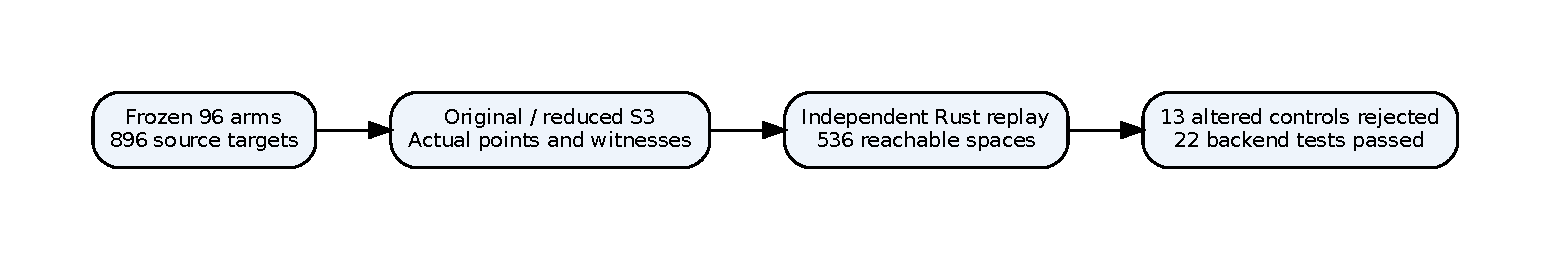
\includegraphics[width=\linewidth]{bridge.pdf}

\textbf{Recorded first-policy values.} The rational collection columns are the
independently replayed finite first-step recurrence solutions. A kernel proof of
the complete stopping-time interpretation is still open. Degree-request units
multiply the named degree by a call; they do not price total computation.
\begin{center}\small\begin{tabular}{llrrrrr}\toprule
Field & Arm & $\Pr(\Delta R>0)$ & $\mathbb E[\Delta R]$ & Mean reduced $D$ & Calls & Reduced degree requests\\\midrule
F43 & main0 & $4/5$ & $4/5$ & $3$ & $35/12$ & $35/4$\\
F43 & twist0 & $3/5$ & $4/5$ & $14/5$ & $10/3$ & $28/3$\\
F13 & main0 & $1$ & $4/3$ & $7/3$ & $2$ & $14/3$\\
F13 & twist0 & $1$ & $4/3$ & $8/3$ & $2$ & $16/3$\\\bottomrule
\end{tabular}\end{center}
All rows above use size-two bases. Original mean degree is 4 in each.
For F43 main0 the base abscissae are (4,13), twist0 (15,17).
Lower per-query degree can coexist with a larger collection-call recurrence.
For size-three bases the cubic membership reduction leaves S3 unchanged, exactly.

\textbf{Flow and corrections.} One full contract was planned; three native attempts
were executed, one completed, two failed, zero interrupted/resumed/excluded.
Attempt01: producer completed, old Rust division used only two base roots and
rejected the size-three invariant (audit101). Attempt02: corrected audit passed,
but the false-row mutation removed an already empty list; strict changed-payload
guard failed (runner2). Attempt03: versioned nonempty-row control passes the full
contract (runner0), all 13 rehashed controls reject101 with no receipt, and all22
backend tests pass. Each source correction was committed before its fresh rerun.
All97 producer files match both earlier attempts byte for byte; the two successful
audit receipts are identical. Failures and exact altered payloads are preserved.

\textbf{Reproduction.} \texttt{run-uniform-yield-v3.sh FRESH\_DIRECTORY}; freeze sources,
use the official branch checkpoint gate and existing local resources. Per-command
cap600s, iteration envelope3600s, two workers. No cap was hit in native runs. No
timing, GAE, S, rho, external-fastest, intrinsic-regularity or F4/F5 claim is made.
\newpage
\begin{center}{\Large All fixed-policy response profiles}\end{center}
\par
\noindent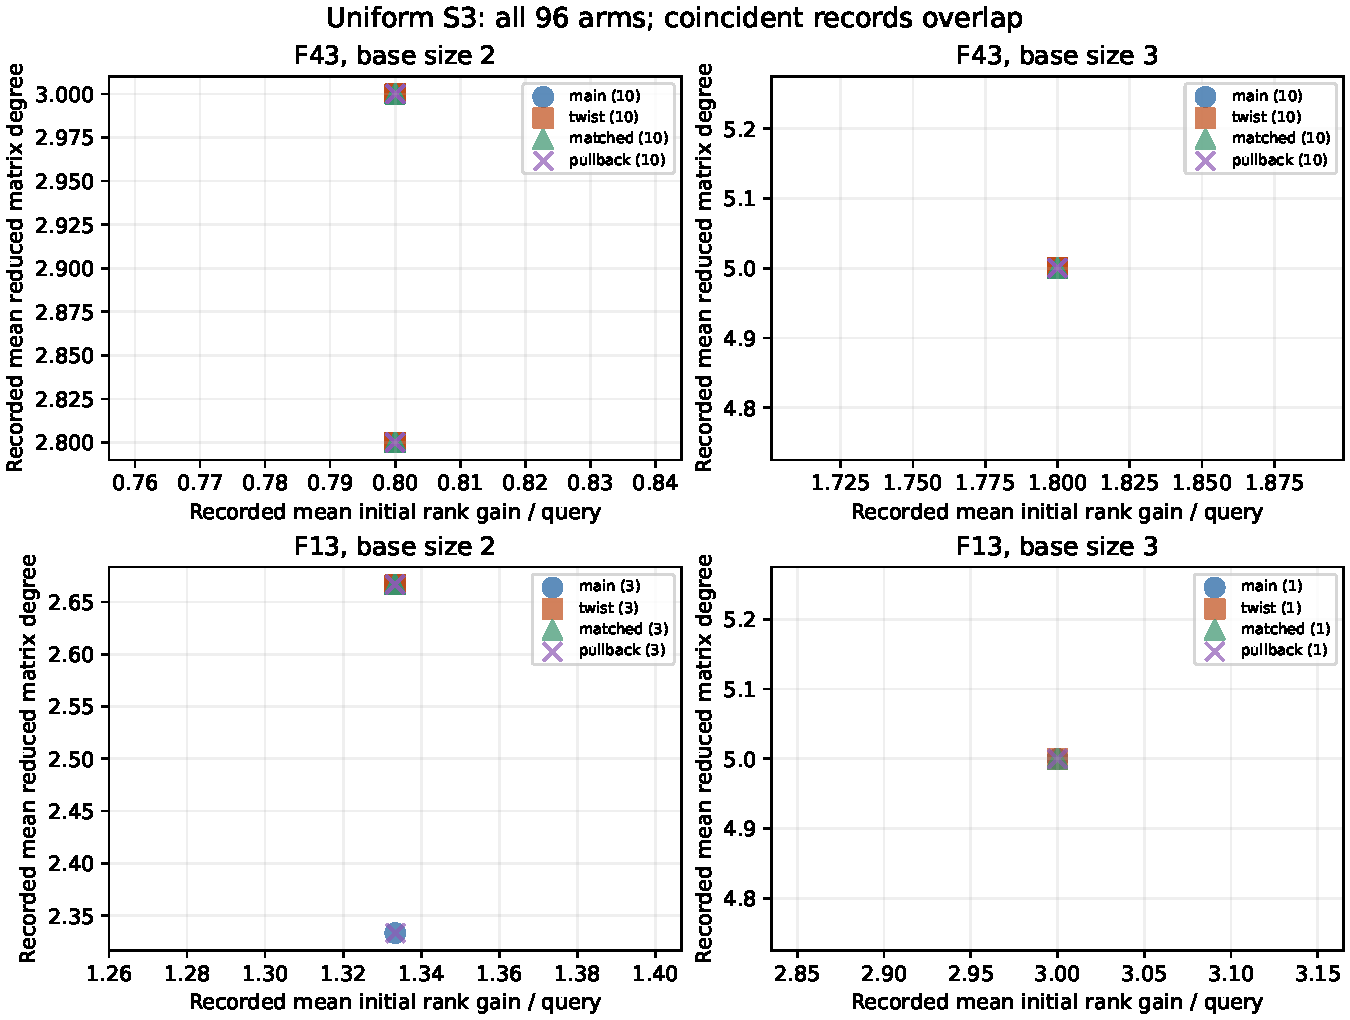
\includegraphics[width=\linewidth]{profiles.pdf}
\textbf{Figure.} Exact finite response averages on all96 arms in \rec. Each panel
retains every increasing base of the indicated size: main, twist, transported
main base and inverse-transported twist base. Coincident points overlap; none
are removed. Fractions are copied from audited records, with decimal conversion
only for plotting. There are no sampling intervals because this is an exhaustive
response census under a declared hypothetical sampler, not a timed random run.

\textbf{Controls and scope.} Matched rows, rank gains, positive probabilities and
collection-call profiles are preserved. Coordinate-dependent solver degrees are
observed rather than assumed invariant. All source logs are derived from actual
public relations; target recovery receives only the point Q. Known labels create
and check public synthetic fixtures outside the recovery interface.

The positive checks cover actual points, root/sign lifting, ideal witnesses,
row spans, promotions, matrices, all reachable spaces/transitions with query
multiplicity, exact rational recurrence solutions, source recovery and frontiers.
Thirteen altered-payload controls cover rows, degree, witness, omitted arm/target,
state transition, rational value, lost query/failed query, log, scalar, source and
frontier. The missing-failed-query control is applicable, not null.

\textbf{Storage.} Canonical97 JSON case files remain loose because the index and
strict auditor name them individually. No case exceeds1MiB. The deterministic raw
archive dehydrates only exact duplicates of these paths and retains every altered
payload; restoration checks all original hashes and repacks identically. Checkpoint
uploads use only the approved branch prefix. No credential is in evidence.
\newpage
\begin{center}{\Large Conditional Lean laws and actual source reductions}\end{center}
The new \path{lean-uniform/UniformCollection.lean} project proves nine named
theorems. The unmodified scoped repository gate passes16 declarations (nine named,
seven generated), zero failing or extra trusted/native axioms. Only
\texttt{propext}, \texttt{Classical.choice}, \texttt{Quot.sound} occur.
Lean4.34.1, Mathlib \path{d13f23b723b8a846827a245b89c10fc7d3f11612}.
The previous208 named/269 audited receipts are historical and are not relabelled
as a fresh combined gate. All17 previous polynomial identities remain unchanged.

Let $N>0$ be the number of query outcomes, $s(L)<N$ the stays, and let $I(L)$
be the improving successor \emph{list with multiplicity}. Heights strictly descend.
If $E,C$ satisfy their explicit terminal and first-step equations, Lean proves
\[
 E(L)=\frac{N+\sum_{M\in I(L)}E(M)}{N-s(L)},\qquad
 C(L)=\frac{D_{\rm mass}}{N}E(L).
\]
It also proves solution uniqueness, scaling, the one-rank-remaining case $E=1/p$,
and the sufficient comparison
\[
 E_T\le E_E,\quad 0\le\bar D_T<\bar D_E,\quad E_E>0
 \quad\Longrightarrow\quad \bar D_T E_T<\bar D_E E_E.
\]
\textbf{Explicit gap.} The first-step equations are hypotheses. This module does
not prove the binding to all536 native subspaces, iid stopping-time semantics,
absorption/integrability, stationary useful yield, or complete work. A larger
initial rank gain alone does not supply the call-count comparison.

\textbf{Actual curves and subgroup maps (historically checked finite bridges).}
F43: E $y^2=x^3+x$, \texttt{icv1-fp6-t0-74779950}; T $y^2=x^3+4x$,
\texttt{icv1-fp6-t0-c6a8a47c}. $P=(31,18)\mapsto U=(24,26)$, order11,
$\phi(x,y)=(41x,11y)$. This fixture is base-field isomorphic.

F13: E $y^2=x^3+x+4$, \texttt{icv1-fp4-t0-6bee67e0};
H $y^2=x^3+4x+7$, \texttt{icv1-fp4-t0-bb514d71};
T $y^2=x^3+4x+6$, \texttt{icv1-fp4-t0-097da6b6}, the $d=2$ monic twist of E.
The executed E--H degree-two coordinate construction followed by scaling5 gives
\[
\Phi(x,y)=\left(12\left(x+\frac2{x-10}\right),
8y\left(1-\frac2{(x-10)^2}\right)\right).
\]
Infinity and $(10,0)$ map to infinity; $P=(0,2)\mapsto U=(8,11)$, order7.
Historical Lean verifies the finite source-scalar equivalence; general geometric
classification is not inferred. Public-base inverse enumeration is setup only.

\textbf{Validation and open holds.} Native replay/controls/backend and the new
scoped Lean gate pass. The fresh root-library outcome is recorded separately in
the validation README; it must not be inferred green from these results. Active
registration is still missing1921 study models; both catalog provenance anchors
and strict membership/byte checks stay. Conductor is unavailable (127), no lease
claimed. General normalization, exceptional S3/S4 lifts, general pairing,
intrinsic regularity, complete calibrated work and PR review/integration remain.

\textbf{Sources checked.} Frozen uniform protocol/correction contracts; S3-yield
and CM8-transfer reports and their point/map proofs; native producer and separate
Rust witness/state implementation; pinned Mathlib and unmodified proof-gate.
Established constrained-Semaev/transported-yield and relation-graph atlas leads
are reused, with no invention claim. The next discriminating step is the actual
state/probability bridge or a preregistered higher-arity constrained system with
exceptional lifting and an actual subgroup reduction; neither is running now.

\end{document}
